% !TeX spellcheck = en_US
\documentclass[a4paper,12pt]{article}

\usepackage{fullpage}
\usepackage[utf8]{inputenc}
\usepackage{fourier}
\usepackage{amsmath}
\usepackage{color}
\usepackage{graphicx}
\usepackage{titlesec}

\titleformat{\section}[hang]{\Large\bfseries}{\Roman{section}\quad}{0pt}{}
\titleformat{\subsection}[hang]{\large\bfseries}{\arabic{subsection}.\quad}{0pt}{}
\titleformat{\subsubsection}[hang]{\large}{\arabic{subsection}\alph{subsubsection})\quad}{0pt}{}

\newcommand{\twodo}[1]{\textcolor{red}{\textbf{todo:} #1}}

\title{\textbf{Exercises for Image Processing 1}\\Problem Sheet 5}
\author{Tim Dobert\\6427948 \and Konstantin M\"ollers\\6313136}

\begin{document}
	\maketitle	
	
	\section{Theoretical Problems}
	\subsection{(Lossless) Image Compression}
	
	\subsubsection{Entropy}
	\subsubsection{Huffman Code}
	
	First of all, we calculate the actual probabilities for the classification in combination with their colors. Because of the independence of these values, we can obtain those just by multiplication.
	
	\begin{table}[h!]
		\centering
		\begin{tabular}{l|l|l|r|l|r}
			$i$ & \textbf{Classification} & \textbf{Color} & \textbf{Probability} $p_i$ & \textbf{Huffman Code} & \textbf{Length} $l_i$ \\\hline
			1 & background & white & 0.900 & \texttt{0} & 1 \\
			2 & print & black & 0.080 & \texttt{10} & 2 \\
			3 & print & red & 0.005 & \texttt{1110} & 4\\
			4 & print & yellow & 0.001 & \texttt{11111} & 5\\
			5 & print & green & 0.002 & \texttt{11110} & 5\\
			6 & print & blue & 0.012 & \texttt{110} & 3\\\hline
			\multicolumn{3}{l|}{$\Sigma$} & 1.000 & \multicolumn{2}{r}{1.131}
		\end{tabular}
	\end{table}
	
	The Huffman code gets calculated by giving the smallest probabilities a binary code (either \texttt{0} or \texttt{1}) and summing up their probabilities. We then compare the sum with other values and iterate. In the end, you get a code The way we calculated the Huffman code is presented in the following schema.
	
	\begin{figure}[h!]
		\centering
		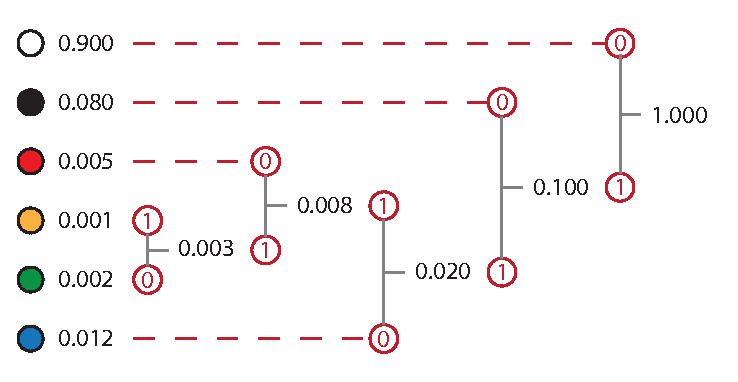
\includegraphics[width=0.7\textwidth]{huffman.pdf}
	\end{figure}
	
	\subsubsection{Mean Length}
	
	To calculate the mean value of our Huffman code, we just need to sum up the probabilities of all pixel values with their code lengths.
	
	\begin{align*}
		\sum\limits_{i = 1}^6 p_i \cdot l_i 	&= 0.900 \cdot 1\\
												&+ 0.080 \cdot 2\\
												&+ 0.005 \cdot 4\\
												&+ 0.001 \cdot 5\\
												&+ 0.002 \cdot 5\\
												&+ 0.012 \cdot 3 = 1.131
	\end{align*}
	
	\subsubsection{Redundancy}
	
	\subsection{Image Segmentation}

	\section{Practical Problems}
	\subsection{(Lossy) Image Compression}
	\subsection{Operators for Edge detection}

\end{document}
